\chapter{Konzeptentwicklung}

Ziel des Konzeptes ist es eine möglichst automatisierte Erstellung digitaler Zwillinge ohne manuelle Interaktion bereitzustellen. Dies bringt verschiedene Vorteile mit sich, vor allem aber, können so dynamisch neue Zwillinge für neue Geräte generiert werden. Dabei ist es auch die Aufgabe bereits bestehende Geräte, im Falle einer Netzwerkpartition wieder mit ihrem entsprechenden Zwilling zu verbinden.\\
Dabei muss berücksichtigt werden, dass verschiedene Services bei dem Erstellen und dem Aufrechterhalten der Verbindung genutzt werden.

Eine wichtige Komponente stellt dabei die \textbf{Device Registry} dar. IBM definiert die Funktion einer Device Registry folgendermaßen:

\begin{definition}[Device Registry]
    \enquote{The Device Registry is the most important part of any IoT solution. With the registry, you can manage your device types and manage, maintain, and monitor the devices that you register.}\autocite{ibm_dr}
\end{definition}

Aus dieser Definition lassen sich mehrere wichtige Eigenschaften entnehmen. Zum einen stellt eine Device Registry einen zentralen Bestandteil dar. Dort liegt die Verwaltung der verscheidenen Geräte, welche alle entweder eigenständig oder miteinander kombiniert zur Erstellung digitaler Zwillinge genutzt werden können. Es geht auch hervor, dass die Art des Gerätes keine Rolle spielt - es können sogar verschiedene Typen verwaltet werden. Gleichzeitig dient es auch als zentrale Anlaufstelle, um die Authentizität von Geräten zu verifizieren. So muss eine Device Registry auch Mechanismen implementierne, der es ermöglicht tausende Geräte zu identifiezieren und zu verwalten.

Alle Bestandteile einer Device-Regisry lassen sich Abbildung \vref{fig:device_registry} erkennen. Von dieser Abbildung lässt sich auch eine exemplarischer Aufbau entnehmen, welche anderen Komponenten eine wichtige Rolle bei der Umsetzung einer Device Registry spielen. Für jeden Anwendungsfall eine eigene Device Registry aufzusetzen, Ressourcen für den Betrieb zu allokieren und zu warten gestaltet sich als unpraktisch. 
Deswegen sind die Registry verschiedener Anbieter \footnotetext{Google IoT Core, IBM, Eclipse Hono} mit einem Namespace System ausgestattet, sodass mehrere Nutzer abgetrennt voneinander innerhalb derselben Registry verwendet werden können.

\begin{figure}
    \centering
    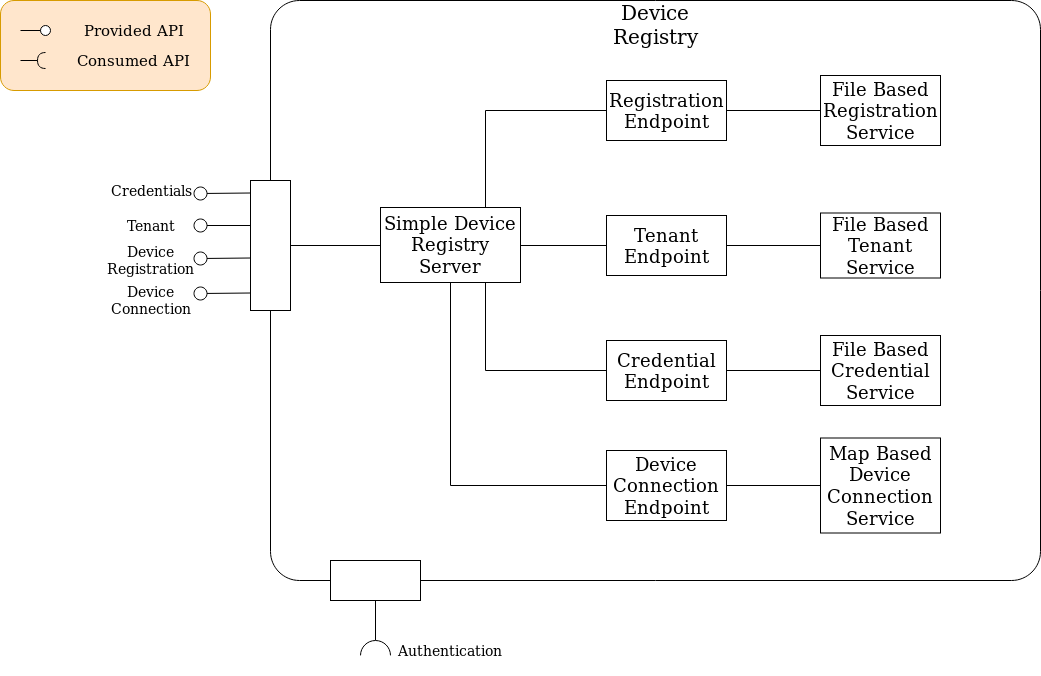
\includegraphics[width=0.75\linewidth]{img/device-registry.png}
    \caption[Bestandteile einer Device Registry]{Beispielhafter Aufbau einer Device Registry am Beispiel von Eclipse Hono. Quelle: \url{https://www.eclipse.org/hono/docs/architecture/component-view/device-registry.png}}
    \label{fig:device_registry}
\end{figure}

Inhärent bedeutet das, dass das Authentifizierungs- und Authorisierungssystem dieses Scoping unterstützen muss. Somit benötigt die Umsetzung der Authentifizierung eine genauere Begutachtung.

\section{Authentifizierung und Authorisierung von IoT Geräten}

Die Authentifizeriung von Geräten im IoT Bereich stellt eine Herausforderung dar. So stellt es sich als sehr unpraktisch dar, für jedes Gerät eigene Zugangsdaten zu generieren und auf dem Gerät zu hinterlegen, damit es sich bei der Device Registry identifizieren kann. Auch stellt es ein Sicherheitsproblem dar, sollten sich Geräte eigenständig in der Device Registry registrieren können, ohne vorher Beweisen zu können, dass sie Zugriff auf einen bestimmten Namespace haben. Es gilt also eine Alternative zu finden, welche es ermöglicht Geräte im großen Stil mit Zugangsdaten auszustatten, welche allerdings nicht Geräteindividuell angepasst werden müssen.

\subsection{Pre-Authentication via Zertifikat}

Um das manuelle Hinterlegen geräteindividueller Zugangsdaten zu vermeiden müssen Alternativen untersucht werden, welche eine Vorauthentifizierung ermöglichen. Grundsätzlich gilt es innerhalb der Kryptographie zwei Formen der Verschlüsselung zu unterscheiden:

\begin{enumerate}
    \item Die \textbf{symmetrische Verschlüsselung}, welche darauf beruht, dass zwei Schlüssel ausgetauscht werden, die im Anschluss genutzt werden können, um eine sichere Kommunikation aufrecht zu erhalten.
    \item  Die \textbf{asymmetrische Verschlüsselung}, die mithilfe eines öffentlichen und eines privaten Schlüssels eine sichere Kommunikation aufbaut und aufrecht erhält.
\end{enumerate}

Ein bekannter Nachteil symmetrischer Verschlüsselungsmethoden, ist der Schlüsselaustausch und das Sicherstellen einer sicheren Kommunikation zwischen einer wachsenden Anzahl an Teilnehmern. Somit wäre eine symmetrische Art der Verschlüsselung suboptimal für einen Anwendungsfall bei digitalen Zwillingen.

Alternativ bieten sich dann noch Möglichkeiten asymmetrischer Verschlüsselungsarten an. Ein Vorteil dieser Art ist es, dass ein Schlüssel austausch sehr einfach erreicht werden kann, da der Aufbau der Verbindung auf Basis eines öffentlichen Schlüssels basiert. Nachteil dieser Methode ist es allerdings, dass der Verbindungsaufbau und die Geschwindigkeit der Verschlüsselung sehr langsam ist. Im speziellen wenn größere Datenmengen verschlüsselt werden müssen sind symmetrische Verschlüsselungen deutlich schneller. Außerdem stellen symmetrische Chiffren ein höheres Sicherheitsniveau zur Verfügung.

Um soviele Vorteile wie möglich bei gleichzeitig so wenig Nachteilen wie nötig zu erhalten, ist es am sinnvollsten beide Ansätze miteinander zu kombinieren. Diese Idee wird bereits in der Internetkommunikation verwendet. Dabei wird mithilfe eines asymmetrischen Schlüsselpaars ein sichere Kanal zur Kommunikation für einen symmetrischen Schlüsselaustausch und die anschließende Verschlüsselung aufgebaut.

Durch den Einsatz eines Zertifikates können die beschriebenen Vorteile erreicht werden.

\subsubsection*{Aufbau eines Zertifikates}
\begin{figure*}
    \begin{verbatim}
    Certificate  ::=  SEQUENCE  {
        tbsCertificate       TBSCertificate,
        signatureAlgorithm   AlgorithmIdentifier,
        signatureValue       BIT STRING  }
    
    TBSCertificate  ::=  SEQUENCE  {
        version         [0]  EXPLICIT Version DEFAULT v1,
        serialNumber         CertificateSerialNumber,
        signature            AlgorithmIdentifier,
        issuer               Name,
        validity             Validity,
        subject              Name,
        subjectPublicKeyInfo SubjectPublicKeyInfo,
        issuerUniqueID  [1]  IMPLICIT UniqueIdentifier OPTIONAL,
                                -- If present, version MUST be v2 or v3
        subjectUniqueID [2]  IMPLICIT UniqueIdentifier OPTIONAL,
                                -- If present, version MUST be v2 or v3
        extensions      [3]  EXPLICIT Extensions OPTIONAL
                                -- If present, version MUST be v3
        }
    
    Version  ::=  INTEGER  {  v1(0), v2(1), v3(2)  }
    
    CertificateSerialNumber  ::=  INTEGER
    
    Validity ::= SEQUENCE {
        notBefore      Time,
        notAfter       Time }
    
    Time ::= CHOICE {
        utcTime        UTCTime,
        generalTime    GeneralizedTime }
    
    UniqueIdentifier  ::=  BIT STRING
    
    SubjectPublicKeyInfo  ::=  SEQUENCE  {
        algorithm            AlgorithmIdentifier,
        subjectPublicKey     BIT STRING  }
    \end{verbatim}
    \caption{Quelle: \fullcite{RFC3280}}
\end{figure*}

...

\begin{figure}
    \centering
    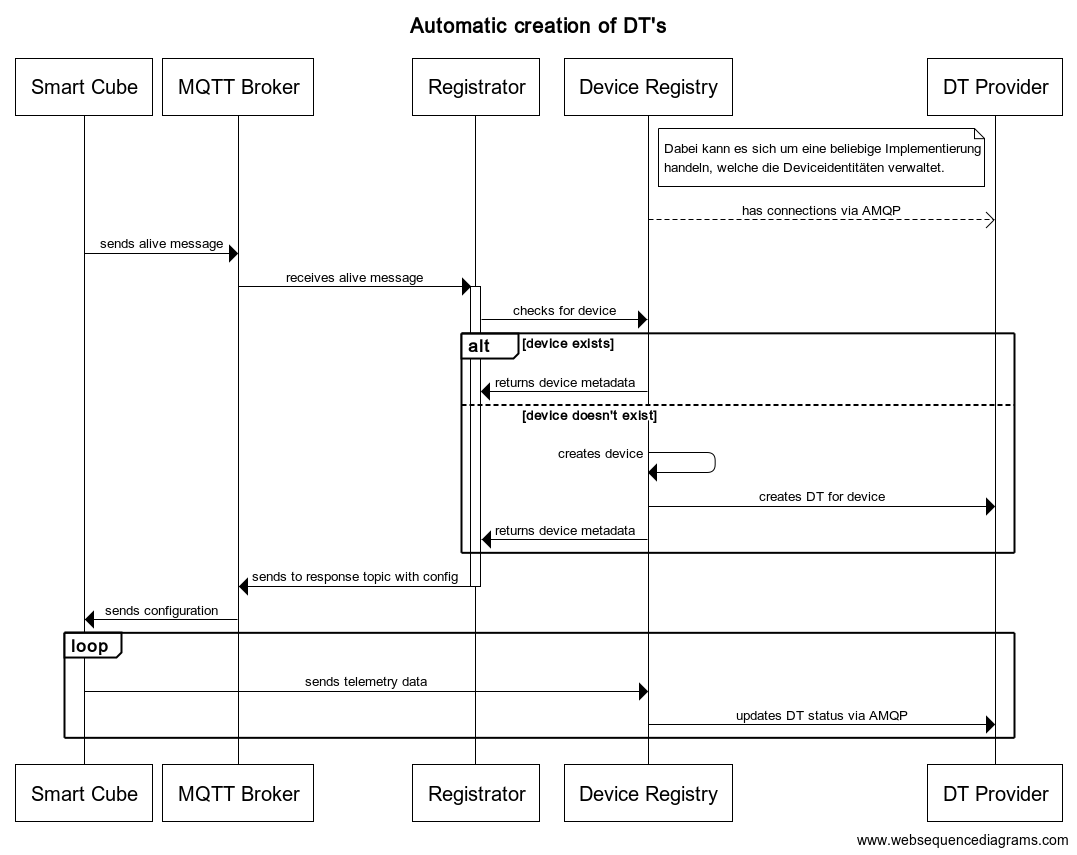
\includegraphics[width=1.0\linewidth]{img/automatic_creation.png}
    \caption[Automatische Erstellung digitaler Zwillinge]{Sequenzdiagramm des Ablaufs, sobald ein Gerät mit einem Netzwerk verbunden ist.\\Quelle: Eigene Darstellung.}
    \label{fig:automatic_creation}
\end{figure}

\begin{enumerate}
    \item Architekturkonzept
    \begin{itemize}
        \item Wieso Device-Registry? Anwendung, Anforderungen, Nutzen, etc.
        \begin{itemize}
            \item Eine Device Registry muss verschiedene Aufgaben erfüllen
            \item Muss Devices registrieren/verwalten können
            \item Verbindungen der Devices müssen abrufbar sein
            \item Authentifizierung/-sinformationen der Devices muss gespeichert werden
            \item bei generischer Nutzung $\rightarrow$ Scoping via namespace/tenant wichtig und muss dem device zugenordnet werden können
        \end{itemize}
        \item Authentifizierung, DaaS(Device as a Service), massenhafte Authentifizierung
        \begin{itemize}
            \item Was für verscheidene Methoden gibt es?
            \item Welche werden verwendet?
            \item Was wäre möglich, wo liegt der aktuelle Stand der Forschung
        \end{itemize}
        \item Common Schnittstellenformate, welche sind im Umlauf wie können sie zusammengeführt werden, sodass alle obigen Anforderungen noch laufen und erfüllt sind?
        \begin{itemize}
            \item Ein wenig die funktionalität und Idee hinter Eclipse Hono erklären. Dabei kurz die Grundlagen jedes Formats erklären
            \item MQTT
            \item AMQP
            \item HTTP
            \item WS (?)
        \end{itemize}
        \item Unterscheidung zwischen einer Device-Registry und der Speicherung als DT
        \begin{itemize}
            \item Hier liegt der Übergang der Arbeit; Es müssen von Geräten in der Device Registy DTs gebildet werden, nach möglichkeit automatisiert, sodass dann Daten des Gerätes übertragen werden
        \end{itemize}
        \item Was muss eine DT-Architektur mit sich bringen, damit Definition erfüllt Ist?
        \begin{itemize}
            \item Hier ein wenig auf die Ditto Idee eingehen.
            \item Konzept hinter Connections erklären; Was sind Connections, Was bringt das an Vorteilen mit sich
            \item Kombination zwischen Device-Registry und DT (hier liegt das Kernproblem!)
        \end{itemize}
        \item verschiedene Zugriffsarten auf die Daten eines DT
        \begin{itemize}
            \item Wie wird das alles exposed in Ditto?
            \item Kommt natürlich auf den Anwendungsfall an
            \item HTTP/WS
            \item AMQP
            \item usw.?
        \end{itemize}
        \item Welche Daten sind vorhanden und wie kann sichergestellt werden, dass ein speziell Modell für DT's vorliegt? $\rightarrow$ Hier kommt dan Vorto ins Spiel. Kurz das Konzept und Idee dahinter erläutern
        \begin{itemize}
            \item Vorto als Strukturregistry.
            \item Wieso ist das so wichtig
            \item welche vorteile gibt es, ein solches ding zu haben
        \end{itemize}
    \end{itemize}
    \item Softwarekonzept
    \begin{itemize}
        \item Müsste nochmal genau abklären, was damit gemeint ist
    \end{itemize}
\end{enumerate}